\documentclass{article}
\usepackage{graphicx}
\begin{document}

\section*{Network Flow 1}

set places := Albany Abq Atlanta Boise Boston Casper Charleston 
              Chicago;
set roues := (Albany,Casper) (Albany,Boise) (Abq,Boise) 
             (Abq,Boston) (Atlanta,Boston) (Atlanta,Chicago) 
             (Boise,Casper) (Boise, Charleston) 
             (Boston, Charleston) (Boston,Chicago);
             
param supply :=
Albany 10000
Abq 7000
Atlanta 9000
Boise 0
Boston 3000
Casper 0
Charleston 0
Chicago 0;

param demand :=
Albany 0
Abq 0
Atlanta 0
Boise 2000
Boston 0
Casper 7000
Charleston 8000
Chicago 6000;

param minimum :=
Albany Casper 3000
Albany Boise 1000
Abq Boise 0
Abq Boston 2000
Atlanta Boston 1000
Atlanta Chicago 500
Boise Casper 1500
Boise Charleston 1000
Boston Charleston 2000
Boston Chicago 1000;

param maximum :=
Albany Casper 6000
Albany Boise 5000
Abq Boise 4000
Abq Boston 7000
Atlanta Boston 5000
Atlanta Chicago 4000
Boise Casper 6000
Boise Charleston 5000
Boston Charleston 7000
Boston Chicago 3000;

param cost :=
Albany Casper .6
Albany Boise .4
Abq Boise .3
Abq Boston .5
Atlanta Boston .2
Atlanta Chicago .125
Boise Casper .25
Boise Charleston .3
Boston Charleston .5
Boston Chicago .2;
Network flow problems are a very important type of linear programming problem.  The idea is we have a set of objects (stores, blogs, nerves in a human body), that can transmit something (goods, information, messages to and from the brain) to other objects in the set.  The connections between objects need not be two-ways: just because object A transmits to object B does not mean B will transmit to A.  A good example of a network flow problem is the Transportation Problem also found in the Pyomo directory.  While a simplified example, it is essentially a problem of moving goods throughout the set of locations so that demand can be satisfied at a few locations.

In that vein, we do a compareable example to begin.  We are looking at a company that produces grain.  There are three mills in the area with a certain supply, and these mills produce goods that they store in two warehouses until they need to be shipped to the three factories with some value for their demand.  The warehouses have no supply or demand.  To make matters more complicated, two of the mills ship directly to the factories.  Another factor to take into account is that each route has a maximum amount that can be shipped along it, which is a realistic condition (if being shipped by train, for example, only so many trains can run in a period of time).  Worse, a company is being contracted to do the shipping, and they require a minimum amount along each route that we must also take into account.  Finally, it costs a certain amount per volume of grain to ship along any route (to pay for space on trains, or gas for cars, for example).  All of this must be taken into account to create a realistic model that will minimize the total cost for shipping grain from the mill to the factory.

The image below shows all the routes in this model, along with their associated costs.

\begin{figure}
\begin{center}
 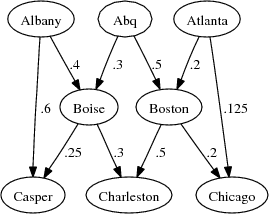
\includegraphics[width=200pt,height=200pt]{NetworkFlow1-crop.png}
 % NetworkFlow2.pdf: 612x792 pixel, 72dpi, 21.59x27.94 cm, bb=0 0 612 792
\end{center}
\caption{A map of the transportation network.  Albany, Albuquerque and Atlanta are the factories, Boise and Boston are warehouses and Casper, Charleston and Chicago are the locations of the stores.}
\end{figure} 

\subsection*{Build the model}

We begin this model as we always do

\begin{verbatim}
from pyomo.core import *

model = AbstractModel()
\end{verbatim}

Now we must define our sets.  In the transportation problem, we had a set for the warehouses and a set for the stores.  In this example, we're going to be more sophisticated: we're going to just have one set for all the locations.  Additionally, we're going to have one set that holds all of the different routes between these locations.  This construction will help later when creating the constraints and is a more typical model for a network flow problem: we care about the nodes and arcs, so it makes sense to make those the sets.  The code is a little different than what we've done before.

\begin{verbatim}
model.places = Set()
model.routes = Set(within=model.places*model.places)
\end{verbatim}

While the definition for the set ``places'' should be familiar, how we defined ``routes'' is a bit more foreign.  By saying \begin{verbatim}within=model.places*model.places\end{verbatim} we mean that routes is a subset of places crossed with itself.  Thus, the set of routes will be a set of tuples, and each part of these tuples will come from the set of places.  This is exactly what we want as each route is uniquely defined by its starting and ending place, so if we have a route (A,B) that just means we can ship grain from place A to place B.  Note, though, that this does not mean we can ship from B to A, that's a different tuple, (B,A).

The parameters are fairly straightforward after this point.  Each place has an associated supply and demand (either or both of which could be $0$), and each route has a minimum and maximum amount that it can be used.  Also, each route has an associated cost with it.  All of these are parameters over one set so the implementation should be routine at this point.

\begin{verbatim}
model.supply = Param(model.places)
model.demand = Param(model.places)
model.cost = Param(model.routes)
model.minimum = Param(model.routes)
model.maximum = Param(model.routes)
\end{verbatim}

Now to define our variables.  We're trying to figure out how much to ship along any route, so creating an amount variable over the set of routes seems logical.  As in the previous examples, we restrict it to non-negative numbers as shipping negative amounts of grain is impossible and illogical.

\begin{verbatim}
model.amount = Var(model.routes, within=NonNegativeReals)
\end{verbatim}

In the transportation problem, we were lucky and (after we added a bit more supply) the total supply was the same as the total demand.  But what if we have more supply than demand?  It would be hard for a user to track down where that extra supply is; they would need to carefully look through each warehouse and store, calculating how much is coming in compared to the location's supply and demand to find where the extra supplies went.  To make it simpler for the user to find the extra amounts, we introduce another variable: excess.  At the end, when we solve the problem, the solution will also include an ``excess'' section that tells us how much grain is left over at each location so we won't lose track of any of our supply, but instead easily and quickly know where it is.  Note that excess is a variable over the locations and shouldn't be negative.  From here, the implementation is similar to the amount variable.

\begin{verbatim}
model.excess = Var(model.places, within=NonNegativeReals)
\end{verbatim}

As in the diet problem and the transportation problem, our goal is to minimize cost.  To calculate the total cost, we just take the amount that will travel along each route, multiply it with the cost to travel that route, and sum all of these values together.  To code it we input

\begin{verbatim}
def costRule(model):
    return sum(model.cost[n]*model.amount[n] for n in model.routes)

model.costTotal = Objective(rule=costRule)
\end{verbatim}

\noindent
Once again, this is just taking the dot product of the cost and amount vectors.  Additionally, recall the being an objective means that Pyomo will try to minimize this value.  Since total cost is our objective, Pyomo will find the least expensive way to ship our goods from the mills to the factories.

One of the main factors outlined above was that we ship a minimum amount on each route, and at the same time we don't exceed a maximum.  We could create two constraints, one that ensures we're above the minimum and another that checks if we're below maximum, but we can easily construct this as one constraint.

\begin{verbatim}
def loadRule(i,j, model):
    return (model.minimum[i,j], model.amount[i,j], 
        model.maximum[i,j])

model.loadOnRoad = Constraint(model.routes, rule=loadRule)
\end{verbatim}

The second line here indicates that the value of amount must be between the minimum and maximum values (inclusive) allowed on that route.  Also, but putting routes as one of the arguments to the constraint we will cycle through every possible route when doing this rule.  Essentially, this is just the cost rule for each individual route compressed into one constraint.  Considering that this one constraint also contains the minimum and maximum load rules, we see that it is very, very useful.

Finally, we have our supply and demand rule.  Like the previous constraint, we can compress supply and demand into one rule.  The basic idea is that the supply, plus whatever flows in, must be greater than or equal to the demand and whatever flows out.  So, our mills will have an initial supply but nothing new will flow in.  Similarly, they have no demand, but a certain amount flowing out.  So for a mill, the supply demand rule requires
$$\textrm{supply} + 0 >= 0 + \textrm{amount leaving mill}$$
Which is a logical constraint.  Similarly, for the factories, which have no initial supply and no flow out, but do have a flow in and demand, the equation might look like
$$0 + \textrm{amount entering factory} >= \textrm{demand} +0$$
The warehouses are a bit more complicated, though, as they might have flow in and out, along with an initial supply or demand (but not both---it can use its supply to meet its own demand).  Thus, this equation might be
$$\textrm{supply} +\textrm{amount entering warehouse} >= 0 + \textrm{amount leaving warehouse}$$

However, we have a further complication.  We included the excess variable, the amount left over at any given place, which isn't described in the equations above.  Rather than inequalities, the above equations should actually be equalities of the form.
$$\textrm{supply} +\textrm{amount in} = \textrm{demand} +\textrm{amount out} +\textrm{amount left over}$$
The implementation of this is a bit more complex than previous constraints.

\begin{verbatim}
def supplyDemandRule(nn, model):
    
    amountIn  = sum(model.amount[i,j] for (i,j) in model.routes 
        if j == nn)
    amountOut = sum(model.amount[i,j] for (i,j) in model.routes 
        if i == nn)
    
    input  = amountIn + model.supply[nn]
    output = amountOut + model.demand[nn] + model.excess[nn]
    
    return input == output

model.supplyDemand = Constraint(model.places, rule=supplyDemandRule)
\end{verbatim}

What we did was just construct a few additional variables; this wasn't required but makes reading and understanding the code much, much simpler.  The variable ``amountIn'' looks at each route to find ones that end in this location, then adds the amount on each of those routes together to determine how much flows to each location.  The ``amountOut'' variable fucntions similarly for the flow out.  Then we just create an ``input'' and ``output'' and ensure they're equal.  As in some of the previous constraints, we feed the set of places into the constraint as an arguement so it will index over that set, and thus this rule functions for all the places in our network.

We have now finished creating the model.  Save this as a .py file before continuing.

\subsection*{Data Entry}

As always, we begin by defining our sets.  The set of places is straightforward with nothing new or different to be considered.

\begin{verbatim}
set places := Albany Abq Atlanta Boise Boston Casper Charleston 
              Chicago;
\end{verbatim}

However, the set of routes is a bit different.  Since it was defined as a set crossed with itself, it's a set of tuples which must be taken into account.  Fortunately, the implementation isn't very complex

\begin{verbatim}
set roues := (Albany,Casper) (Albany,Boise) (Abq,Boise) 
             (Abq,Boston) (Atlanta,Boston) (Atlanta,Chicago) 
             (Boise,Casper) (Boise, Charleston) 
             (Boston, Charleston) (Boston,Chicago);
\end{verbatim}

We now need to input the supply and demand parameters for each location.  We use the same method for inputting parameters over one dimension that we did before in both the diet problem and the transportation problem.

\begin{verbatim}
param supply :=
Albany 10000
Abq 7000
Atlanta 9000
Boise 0
Boston 3000
Casper 0
Charleston 0
Chicago 0;

param demand :=
Albany 0
Abq 0
Atlanta 0
Boise 2000
Boston 0
Casper 7000
Charleston 8000
Chicago 6000;
\end{verbatim}

The last three parameters, minimum and maximum load and cost, are all over the set of routes.  Even though it is a set of tuples, inputting the information is very similar to what was done with supply and demand.  Note how to format the tuples being used to index the parameters.

\begin{verbatim}
param minimum :=
Albany Casper 3000
Albany Boise 1000
Abq Boise 0
Abq Boston 2000
Atlanta Boston 1000
Atlanta Chicago 500
Boise Casper 1500
Boise Charleston 1000
Boston Charleston 2000
Boston Chicago 1000;

param maximum :=
Albany Casper 6000
Albany Boise 5000
Abq Boise 4000
Abq Boston 7000
Atlanta Boston 5000
Atlanta Chicago 4000
Boise Casper 6000
Boise Charleston 5000
Boston Charleston 7000
Boston Chicago 3000;

param cost :=
Albany Casper .6
Albany Boise .4
Abq Boise .3
Abq Boston .5
Atlanta Boston .2
Atlanta Chicago .125
Boise Casper .25
Boise Charleston .3
Boston Charleston .5
Boston Chicago .2;
\end{verbatim}

\noindent
Just put the beginning location, then a space, then the end location with the associated value afterwards.

We've now finished inputting the data, so all that's left is to run the model.  Make sure to save this information as a .dat file.

\subsection*{Solution}

We use Pyomo to generate the results.  Below is a simplified version of Pyomo's output for brevity and ease of reading.

\begin{verbatim}
  Objective: 11575

  Variable: 

    Amount:
    Boise Casper      1500
    Albany Casper     5500
    Abq Boston        2000
    Boise Charleston  1500
    Atlanta Boston    3500
    Albany Boise      1000
    Atlanta Chicago   4000
    Boston Chicago    2000
    Boston Charleston 6500
    Abq Boise         4000

    Excess:
    Albany  3500
    Abq     1000
    Atlanta 1500
\end{verbatim}

There are a few key pieces of information to highlight here.  First, we see that our optimal cost is \$$11,575$, along with the amounts to ship along each route.  For example, we should ship $4000$ units from Albuquerque to Boise.  Additionally, at the bottom we see the values for the ``excess'' variable: Albany will have $3500$ units, Albuquerque will have $1000$ and Atlanta will have $1500$.  If these values are summed, it is $6000$, the exact difference between the total supply and total demand at the start of our model, which is exactly how it should be.  Note also that the excess was just at our initial locations; that doesn't have to be the case.  Depending on how the model was set up, other places may have had an excess---for example if the minimum amount shipped from Albuquerque to Boston was increased, it might shift the excess to Boston.

This was a simple network flow problem.  In the next example, we'll investigate a different kind of network flow problem.

\end{document}
